\DiaryEntry{Permutations, 3 (Number of Fixed Points)}{2016-01-04}{Combinatorics}

Consider a set of \(n\) elements: In total there are \(n!\) permutations - How many permutations are there with \(k\) fixed points? This number is callled
\href{https://en.wikipedia.org/wiki/Rencontres_numbers}{Recontres
Number} and will be denoted as \(D_{n,k}\).

For example \(n=5\) and consider the permutation

\[
\sigma=\begin{pmatrix}
1 & 2 & 3 & 4 & 5 \\
2 & 5 & 3 & 1 & 4
\end{pmatrix}
\]

We have one fixed point: \(\sigma(3) = 3\).

In order for a permutation to have \textbf{one} fixed point, any of the \(n\) elements can become the fixed point. The other \(n-1\) must not have a fixed point, therefore they must form a derangement. There are \(!(n-1)\) such derangements. Therefore, the number of permutations with exactly one fixed point is

\[
D_{n,1} = n !(n-1)
\]

In a similar way we can argue for the number of permutations having two fixed points: There are \(n \choose 2\) ways to select the two fixed points and the other \(n-2\) elements must form a derangement.
Therefore, we have

\[
D_{n,2} = {n \choose 2} !(n-2)
\]

Generalizing, we obtain

\[
D_{n,k} = {n \choose k} !(n-k)
\]

\subsubsection{Some Values}

can be found
\href{https://en.wikipedia.org/wiki/Rencontres_numbers}{here} and are
shown below.

\begin{figure}
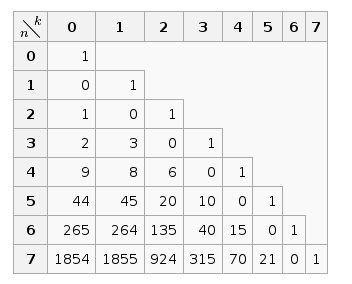
\includegraphics{images/recontres_numbers.png}
\end{figure}

The following properties can be observed:

\begin{itemize}
\item
  It can be seen that \(D_{n,n-1} = 0\); there are no permutations of
  \(n\) elements having \(n-1\) fixed points; the last element must also
  be a fixed point.
\item
  There is one n-permutation with n fixed points: \(D_{n,n} = 1\) which
  is the identity permutation.
\item
  The number of permutations without a fixed point (i.e. \(k=0\)) equals
  the derangements; i.e. \(D_{n,0} = !n\).
\item
  The row-sum equals the number of permutations; i.e.
  \(\sum_{k} D_{n,k} = n!\). We can split the permutations into groups
  having the same number of fixed points. Summing over the group-sizes
  yields the total number of permutations.
\end{itemize}
